\documentclass[cn,10pt,math=newtx,chinesefont=founder]{../elegantbook}

\title{力學題目彙整}
\subtitle{2021年}

\author{李宥頡}
\institute{National Taiwan University}
%\date{May 2, 2021}
%\version{4.1}
%\bioinfo{自定义}{信息}


\setcounter{tocdepth}{3}

%\logo{logo-blue.png}
\cover{cover.jpg}

% 本文档命令
\usepackage{array}
\newcommand{\ccr}[1]{\makecell{{\color{#1}\rule{1cm}{1cm}}}}

\definecolor{customcolor}{RGB}{32,178,170}
\colorlet{coverlinecolor}{customcolor}

\begin{document}

\maketitle
\frontmatter

\chapter*{序}
\tableofcontents

\mainmatter

\chapter{程力}
\section{斜拋}
拋體運動根據運動獨立性(或稱運動重疊原理),可將一曲線運動分為兩個正交方向的直線運動來討論。一般來說,習慣分解成水平方向與鉛直方向,以常見的直角笛卡爾
座標(Cartesian Coordinate),我們將水平方向稱為$x$方向,鉛直方向稱為$y$方向,由於重力恆指向$-y$,故鉛直方向作鉛直上拋運動,且水平方向不受重力,
故水平方向作等速度運動。根據上述,運動的含時參數方程(參數為時間$t$)為
\begin{equation}\label{1.1}
    x = v_0 \cos\theta t\ \ \ \ \ \ \ y = (v_0 \sin\theta)t -\frac{1}{2}gt^2
\end{equation}
\begin{equation}
    v_x = v_0 \cos\theta \ \ \ \ \ \ \ v_y = v_0 \sin\theta - gt
\end{equation}
對於斜拋來說,我們主要對飛行時間$T$、最大高度$H$、水平射程$R$有興趣。直覺上飛行時間應由鉛直方向決定,因為水平方向作等速度運動,看不出時間的影響,故
從鉛直方向的上拋運動判斷。由於上拋上下程的對稱性,飛行時間$T=T_{上}+T_{下}=2T_{上}=\frac{2v_0 \sin\theta}{g}=\frac{2v_{0y}}{g}$。
由於水平方向為等速度運動,水平射程$R = $水平初速 $\times T = \frac{2 v_0 \cos\theta \sin\theta}{g} = \frac{v_0 \sin 2\theta}{g}$。
最後,最大高度$H$由上拋得出,可得$H=\frac{v_0^2 \sin^2\theta}{2g}=\frac{v_{0y}^2}{2g}$。\\
\begin{equation}
\begin{array}{l}
    T = \frac{2v_0 \sin\theta}{g} \\
    R = \frac{v_0 \sin 2\theta}{g} \\
    H = \frac{v_0^2 \sin^2\theta}{2g}
\end{array}
\end{equation}
斜拋重點討論:
\begin{enumerate}
    \item 水平射程$R = \frac{v_0 \sin 2\theta}{g}$在初速$v_0$固定時,
          有一最大值$R_{Max}=\frac{v_0^2}{g}$,
          並發生在$\theta_{Max}=\frac{\pi}{4}$
    \item 同一水平射程$R = \frac{v_0 \sin 2\theta}{g}=\frac{2v_0 \sin \theta \cos \theta}{g}$,
          在固定初速度並透過簡單的代換可知,有兩個拋射角$\theta_1 , \theta_2$滿足同一射程,且
          \begin{equation} \label{1.4}
            \theta_1+\theta_2 = \frac{\pi}{2}
          \end{equation}
\end{enumerate}


\section{斜拋打斜面}
\subsection{運動方程}
在討論斜面上的斜拋運動,我們常選擇平行斜面方向為$x$軸,而垂直斜面方向為$y$軸。分解初速和加速度
之後,此時兩方向的運動均為等加速度運動。\\
\begin{minipage}{\linewidth}
    \begin{minipage}{0.45\linewidth}
\raggedleft
\flushleft
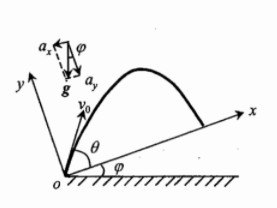
\includegraphics[width=0.5\textwidth]{image/斜拋打斜面.png}
    \end{minipage}
    \hspace{0.05\linewidth}
    \begin{minipage}{0.45\linewidth}
\raggedright
\begin{equation} \label{1.5}
    x = v_0 \cos\theta t\pm \frac{1}{2}(g \sin \varphi) t^2 \ \ \ \ \ \ \ y = (v_0 \sin\theta)t -\frac{1}{2}(g\cos \varphi) t^2
\end{equation}
\begin{equation}
    v_x = v_0 \cos\theta \pm (g \sin \varphi) t \ \ \ \ \ \ \ v_y = v_0 \sin\theta - (g\cos \varphi) t
\end{equation}
    \end{minipage}
\end{minipage}
若欲求斜拋打斜面的射程,即令方程式\ref{1.4}中的$y$為0,求出的$x$值即為射程$R$
\begin{equation}
    R = \frac{2v_0^2 \cos (\theta+\varphi)\sin \theta}{g\cos^2 \varphi}
\end{equation}
在固定$v_0$時,最大射程($+$為向上斜拋,$-$為向下斜拋)
\begin{equation}
    R_{Max}=\frac{v_0^2}{g(1\pm \sin \varphi)}
\end{equation}
和相對應的拋射角($-$為向上斜拋,$+$為向下斜拋)
\begin{equation}
    \theta_{Max} = \frac{\pi}{4} \mp \frac{\varphi}{2}
\end{equation}
\begin{proof}
    \\[20em]
\end{proof}

\begin{note}
    如何找三角函數極值:
    \begin{enumerate}
        \item 利用$\sin$,$\cos$的極值分別發生在$\frac{\pi}{2}$,$0$
        \item 利用三角疊合
        \item 利用和差化積、積化和差轉回1.
        \item 一次微分檢驗
    \end{enumerate}
\end{note}




\section{軌跡方程}
雖然運動方程(即位置與時間的函數關係)已經提供充足的解題要素,在實際處理問題上,
軌跡方程因為消去時間參數$t$,因此在解題上面對不含時的問題中,可以更清楚看到初速與
拋射角的關係。將方程 \ref{1.1}代換
\begin{equation}
    t = \frac{x}{v_0 \cos \theta}
\end{equation}
並代入$y$,即可獲得軌跡方程
\begin{equation}
    y=x \operatorname{tan} \theta-\frac{g x^{2}}{2 v_{0}^{2}\cos^2 \theta}
\end{equation}
利用三角恆等式
\begin{equation}
    1+\tan^2 \theta = \sec^2 \theta 
\end{equation}
代換的原因可以使軌跡方程中的角度,變成單一三角函數$\tan \theta$,方便後續討論
\begin{equation} \label{1.7}
    y=x \operatorname{tan} \theta-\frac{g x^{2}}{2 v_{0}^{2}}\left(1+\operatorname{tan}^{2} \theta\right)
\end{equation}
從方程式\ref{1.7}也可以側面證明出斜拋的確是數學上的拋物線$y = ax^2$,且二次項係數為負,代表開口朝下。
求出軌跡方程可幫助我們探討變數$x,y,v_0,\theta$之間的關係。\\
\begin{enumerate}
    \item 

若假定某斜拋的座標起點為原點$(0,0)$,並且在固定初速度$v_0$,並可通過點$(x, y)$,換句話說,方程
\ref{1.7}當中,只剩$\tan \theta$為變數,且可改寫成$\tan \theta$的二次函數
\begin{equation}
    \operatorname{tan}^{2} \theta-\frac{2 v_{0}^{2}}{g x} \operatorname{tan} \theta+\left(\frac{2 v_{0}^{2}}{g x^{2}} y+1\right)=0
\end{equation}
由二次函數的公式解,可求出$\tan \theta$
\begin{equation}
    \operatorname{tan} \theta=\frac{v_{0}^{2}}{g x} \pm \sqrt{\left(\frac{v_{0}^{2}}{g x}\right)^{2}-\left(\frac{2 v_{0}^{2}}{g x^{2}} y+1\right)}
\end{equation}
一般情況下,$\tan \theta$有兩解,且在斜拋的合理拋射角下(銳角),$\tan \theta$和$\theta$為一對一的函數關係,
即同一位置,在固定初速度之下,有兩個拋射角$\theta_1, \theta_2$對應到此位置,並且我們將證明,若此位置在斜面上
(斜角為$\varphi$),兩拋射角之間有關係(對應方程\ref{1.4},即是$\varphi = 0$的情形)
\begin{equation}
    \theta_1+\theta_2 = \frac{\pi}{2}+\varphi
\end{equation}
\begin{proof}
    \\[20em]
\end{proof}
    \item 在初速度和擊中點的$x$座標固定,最大高度$y_{max}$
    \begin{equation}
        y=y_{\max }=\frac{v_{0}^{2}}{2 g}-\frac{g x^{2}}{2 v_{0}^{2}}
    \end{equation}
    且拋射角$\theta_0$必滿足
    \begin{equation}
        \operatorname{tan} \theta=\operatorname{tan} \theta_{0}=\frac{v_{0}^{2}}{g x}
    \end{equation}
    \begin{proof}
        \\[20em]
    \end{proof}

\end{enumerate}
在斜拋打斜面問題中,主要可以分為兩種方法,第一種利用軌跡方程,解代數問題,此方法時常配合二次函數的
解,討論可行的拋射角。第二種方法是利用向量
\begin{equation}
    \vec{r} = \vec{v_0}t+\frac{1}{2}\vec{g}t^2 
\end{equation}
換句話說,位移向量總是$\vec{v_0}t$和$\frac{1}{2}\vec{g}t^2$兩向量做向量加法,
物理意義相當於先利用$v_0$作等速直線運動,再自由落體$\frac{1}{2}gt^2$,搭配斜面
的幾何,即可利用三角函數的正弦定律求解,見例題2-7。


\section{運動學練習題}

\begin{example}
    電梯以加速度1.22公尺/$秒^2$上升,當上升速度為2.44公尺/秒時,有一螺帽自電梯的天花板上鬆落,
    天花板與升降機的底面相距2.74公尺。請計算
    \begin{enumerate}
        \item 螺帽從天花板落到底面所需的時間
        \item 螺帽相對於電梯外固定柱子的位移和通過的路程
    \end{enumerate}

    \rightline{[練2-2]}
\end{example}
\newpage

\begin{example}
    卡車和汽車在同一車道上,前後均以等速前進,卡車的速度為$v_0$,後面汽車的速度為$3v_0$。由於霧大,能見度低,
    當汽車司機發現卡車時。兩車相距僅為$s_0$,汽車立即制動煞車。已知汽車制動煞車後等減速前進,須經距離$s_1$才
    能停止。試確定兩車不發生碰撞的條件。\\
    \rightline{[練2-3]}
\end{example}
\newpage

\begin{example}
    兩個相同的靜止小球A和B,質量均為$m$,A在B後的距離為a。如A受沿AB方向的沖量I的作用(方向沿AB方向),
    同時B受定力F(沿AB方向)開始運動。試確定A不超越B的條件。\\
    \rightline{[練2-4]}
\end{example}
\newpage

\begin{example}
    在同一起點,用相同大小的初速度以各不相同的拋射角拋出物體,求在同一鉛直面內各拋物線軌跡的最高點所組成的方程。\\
    \rightline{[練2-5]}
\end{example}    
\newpage

\begin{example}
    \begin{enumerate}
        \item 如圖所示,兩質點在地面上同一地點以相同速率$v_0$用不同拋射角$\alpha_1$和$\alpha_2$在同一鉛直面內拋出,作斜上拋運動。試證明
              當兩質點的射程$R$相同時,他們在空中飛行時間的乘積與射程$R$成正比,並忽略空氣阻力。
        \item 如圖所示兩質點在傾角為$\theta$的斜面底部同一位置,以相同的速率$v_0$用與斜面夾角$\alpha_1$和$\alpha_2$向斜面高處拋出,在同一鉛直面作
              斜上拋運動。試證明,當兩質點在斜面上射程$R$相同時,他們在空中飛行時間的乘積與斜面上射程$R$的關係。
        \item 試比較兩者的關係。
    \end{enumerate}
    \rightline{[練2-6]}
\end{example}
\begin{figure}[htbp]
    \flushright
    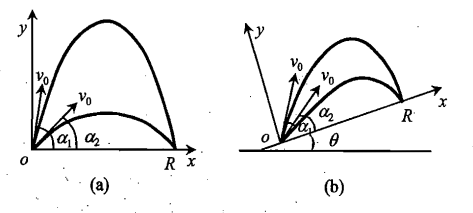
\includegraphics[width=0.3\textwidth]{image/prac_2_6.png}
\end{figure}
\newpage

\begin{example}
    如圖所示,高為$h$的旗竿頂端有一物$P$,一男孩在離旗竿底端A處距離$s$處的O點,欲用彈弓彈射小石塊擊中$P$。已知彈弓彈射出的小石塊初速度為$v_0$,
    問小石塊能擊中$P$的最小$v_0$為何?對應的彈射角應為多大(和水平線的夾角)?\\
    \rightline{[練2-7]}
\end{example}
\newpage

%題目2-8
\begin{example}
    足球運動員在距球門前方$s=11$米處的罰球點,準確地從球門正中橫梁邊沿下踢進一球。橫梁邊沿離地高度$h=2.5$米,足球質量為$m=0.5$千克,空氣阻力不計。求運動員至少要對足球做多少功?
    
    \rightline{[練2-8]}
\end{example}

\begin{solution}

\end{solution}




\newpage

%題目2-9
\begin{example}
    一斜面體兩斜面的傾角分別為$\theta$和$\varphi$,如圖2-練9(a)所示。一物體從傾角為$\theta$的斜面底角處做斜上拋運動。求為使物體從斜面體的頂角處切過,並落在傾角為$\varphi$的斜面底角處,則物體的拋射角$\alpha$與傾角$\theta$、$\varphi$應滿足什麼關係?(用簡單形式寫出。)
    
    \rightline{[練2-9]}
\end{example}

\begin{solution}

\end{solution}


\begin{figure}[htbp]
\flushright
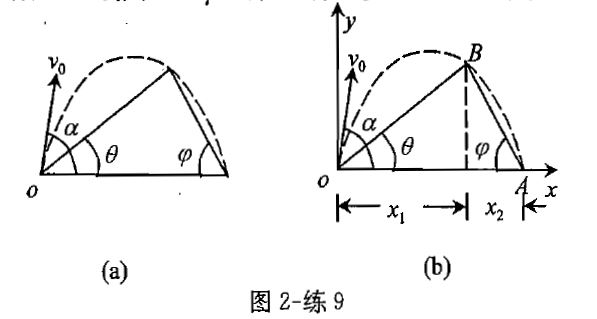
\includegraphics[width=0.5\textwidth]{image/2-9.jpeg}
\end{figure}

\newpage

%題目2-10
\begin{example}
    一輛汽車沿一圓周軌道以$v_0=7.0$米/秒的出速度作勻減速行駛。經過$t_1=5$秒後,汽車的加速度與速度之間的夾角$\theta_1=135^o$。又經過$t_2=3$秒後,其加速度與速度之間的夾角$\theta_2=150^o$。求:(1)圓軌道半徑R;(2)切向加速度的大小$a_\tau$;(3)這兩個時刻($t_1$和$t_1+t_2$時刻)的法向加速度$a_{n1}$和$a_{n2}$。
    
    \rightline{[練2-10]}
\end{example}

\begin{solution}
\begin{enumerate}[label=(\arabic*)]
    \item $R=62.5$米
    \item $a_\tau=0.40$米/秒$^2$
    \item $a_{n1}=0.40$米/秒$^2$,$a_{n2}=0.23$米/秒$^2$
\end{enumerate}
\end{solution}



\newpage

%題目2-11
\begin{example}
    一質點沿圓軌道由靜止開始作勻加速圓周運動。試求此質點的加速度與速度的夾角$\alpha$與其經過的那段圓弧對應的圓心角$\theta$之間的關係。
    
    \rightline{[練2-11]}
\end{example}

\begin{solution}
$tan\alpha=2\theta$
\end{solution}


\newpage

%題目2-12
\begin{example}
    一飛輪的角速度在5秒內由900轉/分均勻地減到800轉/分。求:(1)角加速度$\beta$;(2)在此5秒內的總轉數;(3)再經幾秒,輪將停止轉動。
    
    \rightline{[練2-12]}
\end{example}

\begin{solution}
\begin{enumerate}[label=(\arabic*)]
    \item 角加速度$\beta=-2.09$弧度/秒$^2$
    \item 總轉數$n=70.8$轉
    \item 40秒
\end{enumerate}

\end{solution}




\newpage

%題目2-13
\begin{example}
    有一半徑為R的剛性圓環豎直地在剛性水平地面上作純滾動,圓環中心以不變速度$v_0$在圓環平面內水平向前運動。求圓環上與圓心等高的P點的瞬時速度、切向加速度、法向加速度。如圖2-練13(a)所示。
    
    \rightline{[練2-13]}
\end{example}

\begin{solution}

\end{solution}


\begin{figure}[htbp]
\flushright
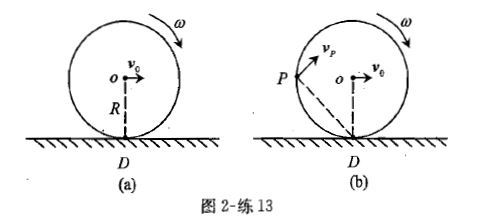
\includegraphics[width=0.6\textwidth]{image/2-13.jpeg}
\end{figure}

\newpage

%題目2-14
\begin{example}
    一質點在半徑為R的圓柱表面等螺距螺旋線上作等速率運動,已知此螺旋線的曲率半徑為$\rho$,質點在垂直於軸平面內的投影的運動週期為T,求質點作此螺旋線運動中沿軸方向的分速度為多大?
    \rightline{[練2-14]}
\end{example}

\begin{solution}

\end{solution}


\newpage

\begin{example}
    小球在豎直平面的 $O$ 點斜向上方拋出,拋射角為 $\theta$,速度大小為 $v_{0}$。
    在此豎直平面 內作 $O M$ 射線與小球拋射方向垂直,如圖 $1-9$ 所示. 小球到達 $O M$ 射線時的速率 
    $v$ 多大?\\
    \rightline{[舒1-4]}
\end{example}
\begin{solution}
    $v_{0} \sqrt{1+4 \cot ^{2} \theta}$
\end{solution}
\begin{figure}[htbp]
    \flushright
    \includegraphics[width=0.3\textwidth]{image/舒1-4.png}
\end{figure}
\newpage

\begin{example}
籃球比賽中,球不經碰撞直接進入籃圈,稱為空心入籃. 運動員在場內某處為使 球能空心入籃,
需要掌握球的拋射角 $\theta$ 和球的初速率 $v$. 實現空心籃的 $(\theta, v)$ 解並不唯一. 
引入最佳拋射角 $\theta_{0}$ (對應的初速率記為 $v_{0}$ ),意即在 $\theta_{0}$ 附近
運動員由於拋射角 $\theta_{0}$ 掌握不夠精確而產生小偏離量 $\Delta \theta$ 時
,為使球能空心入籃,需調整的 $v_{0}$ 偏移量 $\Delta v$ 為最小.某運動員站在 3 分線處立定投籃, 
3 分線與籃圈中心線間的水平距離為 $6.25 \mathrm{~m}$,籃圈離地高度 $3.05 \mathrm{~m}$, 
運動員投籃時出射點的高度為 2.23 $\mathrm{~m}$. 求最佳拋射角 $\theta_{0}$ 和對應的初速率 $v_{0}$.
\end{example}
\begin{solution}
    
\end{solution}


\chapter{隨手筆記}
\section{運動學}
時間的測量
\begin{enumerate}
    \item 測量$\pi$介子壽命,$\pi$介子在感光乳劑中產生並在其中留下細微的痕跡,用顯微鏡觀察,平均而言一個$\pi$
          介子在蛻變之前錒於走過了$10^-7 m$,且速度接近於光速,因此其壽命總共只有$10^-16 s$。(程力)
\end{enumerate}
\chapter{家教問題}
\section{力學}

\begin{example}
    如右圖,OD是水平面,AB和AC皆為斜面,斜角分別為$\theta_1 = 37^\circ$和$\theta_2 = 30^\circ$。一質點由A靜止,經斜面AB滑下,最後靜止於D,若
    改給予、一部為零的初速度$v_0$,經斜面AC滑下(斜面與平面皆有摩擦,且質點與接觸面間摩擦係數皆為$\mu$),則:
    \begin{enumerate}[label=(\Alph*)]
        \item 不論$v_0$為何,皆靜止於D點左側
        \item 不論$v_0$為何,皆靜止於D點右側
        \item 不論$v_0$為何,皆靜止於D點
        \item 若$\mu$同時變大,則必靜止於D點左側
        \item 若$\mu$同時變大,則必靜止於D點右側
    \end{enumerate}
\end{example}



\chapter{大題典}
\section{質點運動學}

%第二章:質點運動學
\begin{example} 
    質量為M的人通過質量可以不計、不可伸長的繩子和摩擦可忽略的定滑輪,將質量為m的重物提起,如圖2.1所示。分兩種情況:(1)物體勻速上升;(2)物體以加速度a上升。求人對地面的壓力。
    
    \rightline{[2.1.1]}
\end{example}

\begin{solution}
\begin{enumerate}[label=(\arabic*)]
\item $N=(M-m)*g$
\item $N=(M-m)*g+ma$
\end{enumerate}
\end{solution}

\begin{figure}[htbp]
\flushright
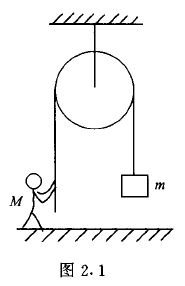
\includegraphics[width=0.3\textwidth]{image/2.1.JPG}
\end{figure}

\newpage


\begin{example} 
    圖2.2中人的質量$m_1=60$kg,人所站著的底板質量$m_2=20$kg,繩子和滑輪質量均可忽略不計。人要用多大的力拉住繩子,才能保持自己和底板靜止不動。
    
    \rightline{[2.1.2]}
\end{example}

\begin{solution}
98N,方向相下
\end{solution}

\begin{figure}[htbp]
\flushright
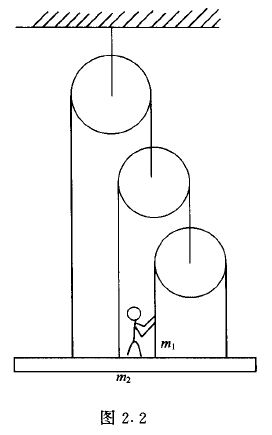
\includegraphics[width=0.4\textwidth]{image/2.2.JPG}
\end{figure}

\newpage


\begin{example} 
    跨過一個無摩擦定滑輪的一根繩子,一端掛有9kg質量,另一端掛有7kg質量,如圖2.3所示。求加速度和繩中的張力。
    
    \rightline{[2.1.3]}
\end{example}

\begin{solution}
加速度$a=1.225m/s^2$,張力$T=77.2N$
\end{solution}

\begin{figure}[htbp]
\flushright
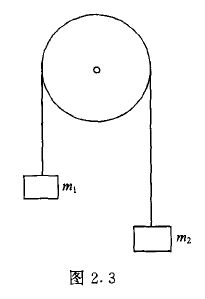
\includegraphics[width=0.3\textwidth]{image/2.3.JPG}
\end{figure}

\newpage


\begin{example} 
    圖2.4中滑輪和繩子質量均可忽略不計,所有的接觸均是光滑的,分兩種情況:(1)要使$m_1$、$m_2$、M之間無相對運動;(2)要使M保持靜止,必須施以M的水平力F多大?M對水平面的壓力N多大?
    
    \rightline{[2.1.4]}
\end{example}

\begin{solution}
\begin{enumerate}[label=(\arabic*)]
\item $F=\frac{m_2(m_1+m_2+M)g}{m_1}$,$N=(m_1+m_2+M)g$
\item $F=\frac{m_1m_2g}{m_1+m_2}$,$N=(M+m_1+\frac{m_1m_2}{m_1+m_2})g$
\end{enumerate}
\end{solution}

\begin{figure}[htbp]
\flushright
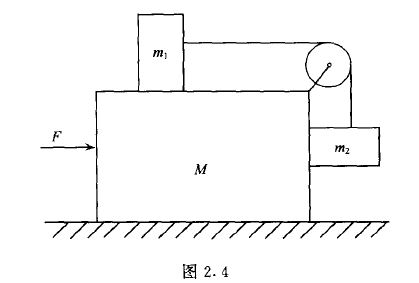
\includegraphics[width=0.6\textwidth]{image/2.4.JPG}
\end{figure}

\newpage

    
\begin{example} 
    圖2.5中小車質量M、重物質量m以及固定斜面的傾角$\alpha$都是已知的,繩子不可伸長,繩子和滑輪的質量以及整個裝置中的摩擦力均可略去不計,求小車和重物的加速度。
    
    \rightline{[2.1.5]}
\end{example}

\begin{solution}
\begin{enumerate}[label=(\arabic*)]
\item $a_M = \frac{4m-Msin\alpha}{M+16m}g$
\item $a_m = \frac{4(4m-Msin\alpha)}{M+16m}g$
\end{enumerate}
\end{solution}

\begin{figure}[htbp]
\flushright
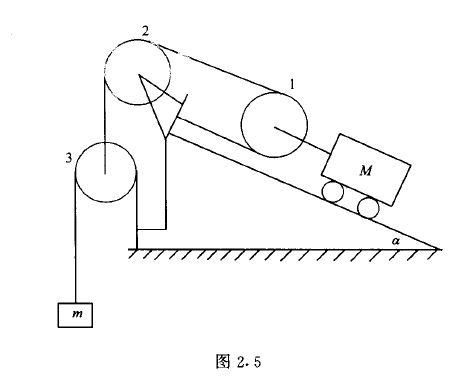
\includegraphics[width=0.7\textwidth]{image/2.5.JPG}
\end{figure}

\newpage


\begin{example} 
    三塊質量均為m的相同物塊疊放在水平面上,如圖2.6所示。各接觸面間的摩擦因數均為$\mu$,有一從零不斷加大的水平力F作用在最下面的物塊上。問F達多大時,最下面的物塊才能有對上面兩物塊的相對運動。
    
    \rightline{[2.1.6]}
\end{example}

\begin{solution}
F略大於$6\mu mg$
\end{solution}

\begin{figure}[htbp]
\flushright
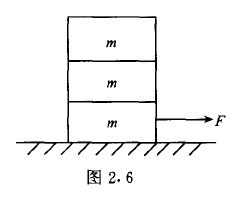
\includegraphics[width=0.3\textwidth]{image/2.6.JPG}
\end{figure}

\newpage


\begin{example} 
    質量為M的木板靜置於水平桌面上(如圖2.7所示),一端A與桌邊對齊,木板上放著一質量為m的小物體,它離板的A端距離l,桌面長L。現在板的另一端B有一恆定的水平力F作用,要將木板從小物體下抽出,又不至於使小物體從桌邊落到地上。各接觸面的摩擦因數均為$\mu$,F至少多大?
    
    \rightline{[2.1.7]}
\end{example}

\begin{solution}
$F_{min} = 2\mu g\frac{(M+m)L-ml}{L-l}$
\end{solution}

\begin{figure}[htbp]
\flushright
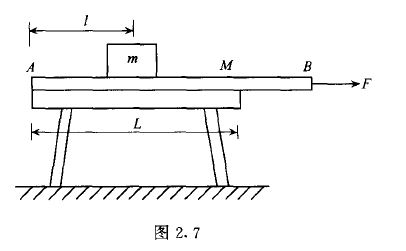
\includegraphics[width=0.6\textwidth]{image/2.7.JPG}
\end{figure}

\newpage


\begin{example} 
    一塊磚以初速度$1.5m/s$在一水平面成$30^o$角的斜面上運動,摩擦因數$\mu = \frac{\sqrt{3}}{12}$。問經1.5s後,此磚離它的初始位置多遠?
    
    \rightline{[2.1.8]}
\end{example}

\begin{solution}
0.064m
\end{solution}

\newpage


\begin{example} 
    兩個無質量的小環在一個處於鉛錘面內的光滑圓環上滑動,一穿過兩環的光滑弦線上帶有三個重物,兩個在兩端,一個在兩環之間。如果當小環A、B在離開圓環最高點H對環心O的張角$30^o$時處於平衡,如圖2.8所示。求繫在弦線上的三重物D、E、G的質量之間的關係。
    
    \rightline{[2.1.9]}
\end{example}

\begin{solution}
D、E、G三重物的質量都相等
\end{solution}

\begin{figure}[htbp]
\flushright
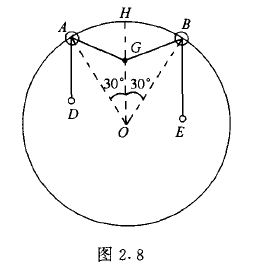
\includegraphics[width=0.3\textwidth]{image/2.8.JPG}
\end{figure}

\newpage


\begin{example} 
    質量為m的小環套在繩上,繩子跨過定滑輪並在另一端繫一質量為M的物體,若繩子不可伸長、質量不計,繩子與滑輪間的摩擦力可忽略,小環相對於繩子以加速度a下落,球小環與繩子間的摩擦力。
    
    \rightline{[2.1.10]}
\end{example}

\begin{solution}
$f = \frac{mM}{m+M}(2g-a)$
\end{solution}

\begin{figure}[htbp]
\flushright
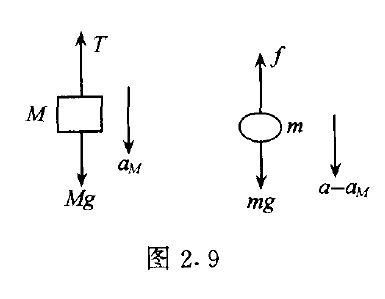
\includegraphics[width=0.4\textwidth]{image/2.9.JPG}
\end{figure}

\newpage


\begin{example} 
    一質量為m的物體通過一根質量可以不計的繩子繞水平棒$1\frac{1}{4}$周後於另一端加一水平力F,如圖2.10所示。若繩子和棒之間的摩擦因數為$\mu$,要使物體保持靜止狀態,應施加多大的水平拉力?
    
    \rightline{[2.1.11]}
\end{example}

\begin{solution}
施加的水平力F:$mge^{-\frac{5}{2}\mu\pi} < F < mge^{\frac{5}{2}\mu\pi}$
\end{solution}

\begin{figure}[htbp]
\flushright
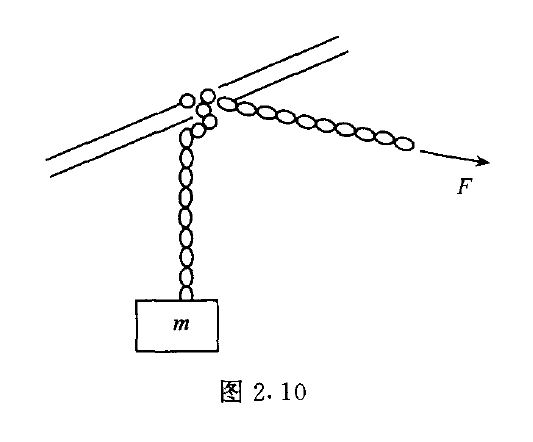
\includegraphics[width=0.4\textwidth]{image/2.10.JPG}
\end{figure}

\newpage


\begin{example} 
    一根質量為M的均質繩子,兩端固定在同一高度的兩個釘子上,在其中點掛一質量為m的物體。設$\alpha$、$\beta$分別為在繩子中點和端點處繩子的切線方向與豎直方向的夾角,如圖2.13所示。證明:$\frac{tan\alpha}{tan\beta} = \frac{M+m}{m}$
    
    \rightline{[2.1.12]}
\end{example}

\begin{solution}
設繩子中點處張力為$T_1$,釘子處繩子張力為$T_2$,連結物體的那段不計質量的繩子張力$T=mg$。\\
對繩子中點和對繩子、物體作為系統平衡方程,\\
$2T_1cos\alpha = mg$ (1)\\
$2T_2cos\beta = (M+m)g$ (2)\\
再對釘子至中點半條繩子列水平方向的平衡方程,\\
$T_2sin\beta = T_1sin\alpha$ (3)\\
由式(1)、(2)得$\frac{T_2cos\beta}{T_1cos\alpha} = \frac{M+m}{m}$\\
由(3)式得$\frac{T_2}{T_1} = \frac{sin\alpha}{sin\beta}$\\
代入上式即得$\frac{tan\alpha}{tan\beta} = \frac{M+m}{m}$
\end{solution}

\begin{figure}[htbp]
\flushright
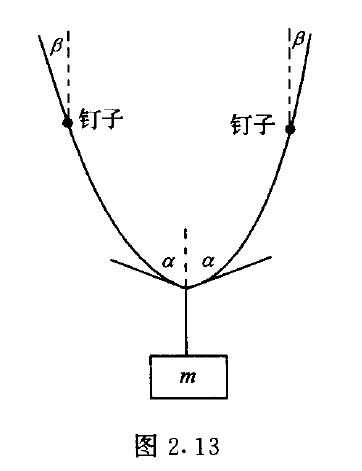
\includegraphics[width=0.3\textwidth]{image/2.13.JPG}
\end{figure}

\newpage


\begin{example} 
    一質量為M的均質鏈條套在一表面光滑、頂角為$\alpha$、底面處於水平的正圓錐上保持靜止,若鏈條平面平行於水面,求鏈條中的張力。
    
    \rightline{[2.1.13]}
\end{example}

\begin{solution}
$T = \frac{Mg}{2\pi}cot\frac{\alpha}{2}$
\end{solution}

\newpage


\begin{example} 
    真空中有缺陷的﹑質量為950kg的衛星,被飛船用一根50m長、線密度為1$kg/m$的均質繩牽著以5$m/s^2$的加速度做勻加速直線運動:
    \begin{enumerate}[label=(\arabic*)]
    \item 飛船作用在繩上的力有多大?
    \item 計算繩的張力;
    \item 飛船上的人精疲力竭睡著了,飛船助推器的控制電路之一發生短路,使加速度變為1$m/s^2$的減速度,這個事故會發生什麼後果?
    \end{enumerate}
    
    \rightline{[2.1.14]}
\end{example}

\begin{solution}
\begin{enumerate}[label=(\arabic*)]
\item $F = 5*10^3$ (N)
\item $T(x) = 5*10^3 - 5x$ (N),$0 \leq x \leq 50$ 
\item 事故發生後10s,衛星與飛船將發生碰撞。考慮到繩子張力的作用,不到10s就發生碰撞。
\end{enumerate}
\end{solution}

\newpage


\begin{example} 
    某人觀察到一空間站始終停留在地球同一點的垂直上空,問觀察者位於地球的什麼地方?盡可能詳細地描述一下此空間站的軌道。
    
    \rightline{[2.1.15]}
\end{example}

\begin{solution}
相對地球不動的空間站在地心平動參考系中的軌道只能位於赤道平面上,部能位於緯度不為零的平面上,因此,看到空間站在垂直上空不動的觀察者必在地球赤道上的某個地方。\\
空間站在位於赤道地面垂直上空的高度$h = 3.59*10^7$ (m)
\end{solution}

\newpage


\begin{example} 
    公園裡有一種轉動水平圓盤,孩子可以做在盤面上任何地方,當盤開始加快轉速時,如果摩擦力不夠大,孩子就可能滑出去。設孩子的質量為50kg,摩擦因數為0.4,盤的角速度為2$rad/s$,問孩子坐在盤上不被滑開的最大半徑有多大?
    
    \rightline{[2.1.16]}
\end{example}

\begin{solution}
$R = 0.98$ (m)
\end{solution}

\newpage


\begin{example} 
    一小物體放在一半徑為R的水平圓盤上,小物體與圓盤間的靜摩擦因數為$\mu$。若圓盤繞其軸的角速度逐一增大到一個值時,小物體滑出圓盤並最終落到比盤面低h的地面上。問從它離開圓盤的那一點算起,小物體越過的水平距離有多大?
    
    \rightline{[2.1.17]}
\end{example}

\begin{solution}
$l = \sqrt{2\mu Rh}$
\end{solution}

\newpage


\begin{example} 
    太陽離銀河系中心大約相距$2.5*10^4$光年,近似地以$1.7*10^8$年的周期繞此中心作圓周運動,地球離太陽的距離為8光分。用以上數據,求出以太陽質量作為單位的銀河系的近似質量。假定作用在太陽上的引力近似為銀河系質量集中在其中心時對太陽的引力。
    
    \rightline{[2.1.18]}
\end{example}

\begin{solution}
M為銀河系質量,$m_s$為太陽質量。\\
$\frac{M}{m_s} = 1.53*10^{11}$
\end{solution}

\newpage


\begin{example} 
    用以下近似數據計算地球和太陽的平均密度之比:
    \begin{enumerate}[label=(\arabic*)]
    \item $\theta$從地球上看太陽的角直徑,$\theta = 0.5^o$;
    \item l為地球表面上緯度為$1^o$的長度,$l = 100$km;
    \item t為地球公轉周期,$t = 1$年$ = 3*10^7$s;
    \item g為重力加速度,$g = 10ms^{-2}$。
    \end{enumerate}
    
    \rightline{[2.1.19]}
\end{example}

\begin{solution}
3.3
\end{solution}

\newpage


\begin{example} 
    \begin{enumerate}[label=(\arabic*)]
    \item 一個均質的球形物體以$\omega$繞對稱軸轉動,如果僅僅靠自身的萬有引力阻礙球體的離心分解,該物體必須具有的最小密度有多大?用這一點估計巨蟹座中轉速為每秒30轉的脈衝星的最小密度。(這是在公元1054年在中國廣泛地被觀察到的一個超新星爆發的遺跡!)
    \item 如果脈衝星的質量與太陽的質量相當,約為$2*10^{30}$kg,這個脈衝星的最大可能半徑多大?
    \item 若脈衝星的密度與核物質的密度相當,它的半徑多大?
    \end{enumerate}
    
    \rightline{[2.1.20]}
\end{example}

\begin{solution}
 \begin{enumerate}[label=(\arabic*)]
\item $\rho_{min} = 1.27*10^{14}$ ($kg/m^3$)
\item $R = 1.55*10^5$ (m)
\item $R = 1.3*10^4$ (m)
\end{enumerate}
\end{solution}

\newpage


\begin{example} 
    一頂角為$2\alpha$($\alpha < 45^o$)的倒立的圓錐面,以恆定角速度$\omega$繞其對稱軸旋轉,在內表面上距軸為r處有一質點,若質點與錐面間的摩擦因數為$\mu$,要使質點相對錐面靜止,$\omega$應處於什麼範圍內?
    
    \rightline{[2.1.21]}
\end{example}

\begin{solution}
$0 \leq \omega \leq \sqrt{\frac{g}{r}\frac{cos\alpha+\mu sin\alpha}{sin\alpha-\mu cos\alpha}}$
\end{solution}

\begin{figure}[htbp]
\flushright
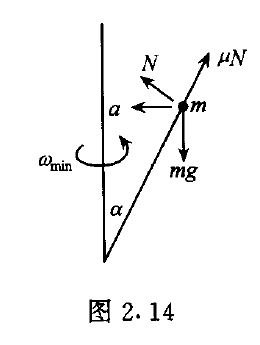
\includegraphics[width=0.3\textwidth]{image/2.14.JPG}
\end{figure}

\newpage


\begin{example} 
    一圓柱形剛性杆上套一質量為m的小杯,杆繞通過一端的固定豎直軸以恆定角速度$\omega$旋轉,旋轉時杆與豎直軸的夾角為$\alpha$。若小環與杆間的摩擦因數為$\mu$,以小環距杆的固定端的距離x為座標列出小環的運動微分方程。
    
    \rightline{[2.1.22]}
\end{example}

\begin{solution}
$m\Ddot{x} = -mgcos\alpha - \mu N + m\omega^2xsin^2\alpha$ ($\Dot{x}>0$時)\\
$m\Ddot{x} = -mgcos\alpha + \mu N + m\omega^2xsin^2\alpha$ ($\Dot{x}<0$時)\\
$N_1 = mgsin\alpha + m\omega^2xsin\alpha cos\alpha$\\
$N_2 = 2m\omega \Dot{x}sin\alpha$\\
$N = \sqrt{{N_1}^2 + {N_2}^2}$
\end{solution}

\begin{figure}[htbp]
\flushright
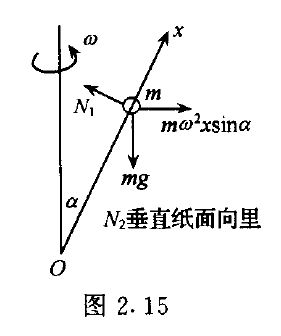
\includegraphics[width=0.3\textwidth]{image/2.15.JPG}
\end{figure}

\newpage


\begin{example} 
    質量為m的小球通過一根原長為l、勁度係數為k的彈性繩繫在光滑的水平檯面上的P點,水平檯面繞離P點距離為b的固定豎直軸以恆定的角速度$\omega$轉動。列出小球在彈性繩拉質狀態下的運動微分方程。
    
    \rightline{[2.1.23]}

\end{example}

\begin{solution}
$m(\Ddot{r} - r{\Dot{\varphi}}^2) = -k(r-l) + m\omega^2(r+bcos\varphi) + 2m\omega r\Dot{\varphi}$\\
$m(r\Ddot{\varphi} + 2\Dot{r}\Dot{\varphi}) = -m\omega^2bsin\varphi - 2m\omega \Dot{r}$
\end{solution}

\begin{figure}[htbp]
\flushright
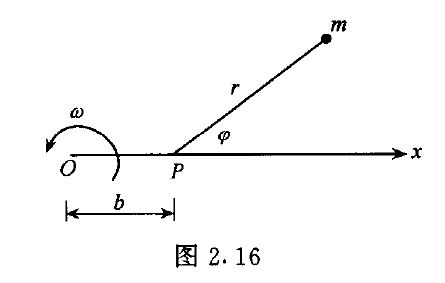
\includegraphics[width=0.4\textwidth]{image/2.16.JPG}
\end{figure}

\newpage


\begin{example} 
    質量為M的斜劈放在摩擦因數為$\mu$的粗糙水平面上,質量為$m_1$的物體用不計質量﹑不可伸長的弦線掛起並跨過固連於斜劈的光滑滑輪與在無摩擦的斜劈面上滑動的質量為$m_2$的物體相連,斜劈面的傾角為$\theta$。如圖2.17所示。
    \begin{enumerate}[label=(\arabic*)]
    \item 求當$\mu$非常大時$m_1$和$m_2$的加速度以及弦線的張力;
    \item 求使斜劈能保持靜止的最小摩擦因數;
    \item 若$\mu$不夠大,斜劈不能保持靜止,有向左的加速度$a_M$,求此$a_M$,列出足夠的方程即可,不必解出$a_M$。設滑輪很小,$m_1$﹑M緊靠時,連結$m_1$的弦線仍可視為在豎直方向。
    \end{enumerate}
    
    \rightline{[2.1.24]}
    
\end{example}

\begin{solution}
\begin{enumerate}[label=(\arabic*)]
\item $a = \frac{m_1 - m_2sin\theta}{m_1+m_2}g$,$T = \frac{m_1m_2}{m_1+m_2}(1+sin\theta)g$
\item $\mu_{min} = \frac{m_2cos\theta \left| m_2sin\theta - m_1 \right|}{M(m_1+m_2) + 2m_1m_2(1+sin\theta) + {m_2}^2cos^2\theta}$
\item $m_1a_{m1} = T - m_1g$ \\ $N_1 - m_1a_M = 0$ \\ $Ma_M = N_2sin\theta - N_1 - Tcos\theta - \mu N$ \\ $N - Mg - T - Tsin\theta - N_2cos\theta = 0$ \\ $m_2a_{m2} = m_2a_Mcos\theta + m_2gsin\theta - T$ \\ $N_2 + m_2a_Msin\theta - m_2gcos\theta = 0$ \\ $a_{m1} = a_{m2}$
\end{enumerate}
\end{solution}

\begin{figure}[htbp]
\flushright
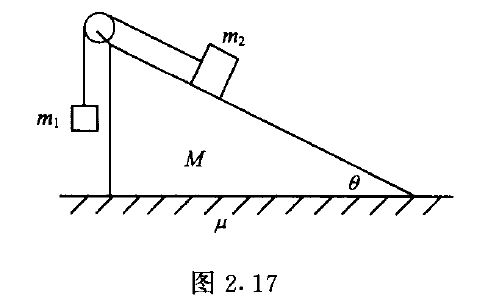
\includegraphics[width=0.4\textwidth]{image/2.17.JPG}
\end{figure}

\newpage


\begin{example} 
    一質量為M的﹑上表面水平的楔形物體,在傾角為$\alpha$的固定的光滑斜面上運動,楔形物體上放一質量為m的質點,如圖2.20所示。若m﹑M間無摩擦,求:
    \begin{enumerate}[label=(\arabic*)]
    \item m相對於M的加速度;
    \item M對斜面的壓力。
    \end{enumerate}
    
    \rightline{[2.1.25]}
    
\end{example}

\begin{solution}
\begin{enumerate}[label=(\arabic*)]
\item $a_{mM} = \frac{(M+m)gsin\alpha cos\alpha}{M+msin^2\alpha}$
\item $N = \frac{M(M+m)gcos\alpha}{M+msin^2\alpha}$
\end{enumerate}
\end{solution}

\begin{figure}[htbp]
\flushright
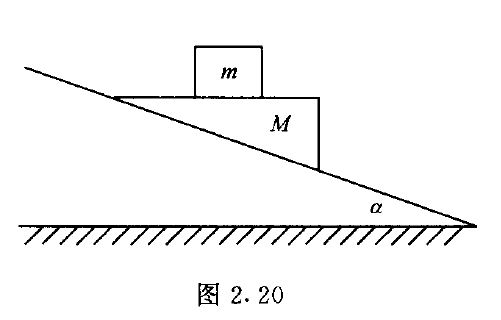
\includegraphics[width=0.4\textwidth]{image/2.20.JPG}
\end{figure}

\newpage


\begin{example} 
    圖2.22中水平桌面上的滑塊質量為M,一條其兩端分別繫著質量為$m_1$﹑$m_2$的兩物體的不計質量﹑不可伸長的細繩套在滑塊上,滑塊、繩子與桌面相互間均無摩擦。試證明滑塊的加速度為\\$a = \frac{4m_1m_2}{M(m_1+m_2)+4m_1m_2}g$
    
    \rightline{[2.1.26]}
    
\end{example}

\begin{solution}
設繩子張力為T,$m_1$﹑$m_2$的加速度為$a_1$﹑$a_2$,均豎直向下,滑塊的加速度為a。\\
$m_1a_1 = m_1g - T$\\
$m_2a_2 = m_2g - T$\\
$Ma = 2T$\\
從桌的邊緣向下取$x_1$﹑$x_2$表示$m_1$﹑$m_2$的座標,沿桌面取x表示M的座標,由於繩長一定,$x_1+x_2+2x = $常量,$a_1+a_2-2a = 0$\\
上述四式含4個未知量T﹑$a_1$﹑$a_2$﹑a,可解出\\
$a = \frac{4m_1m_2}{M(m_1+m_2)+4m_1m_2}g$
\end{solution}

\begin{figure}[htbp]
\flushright
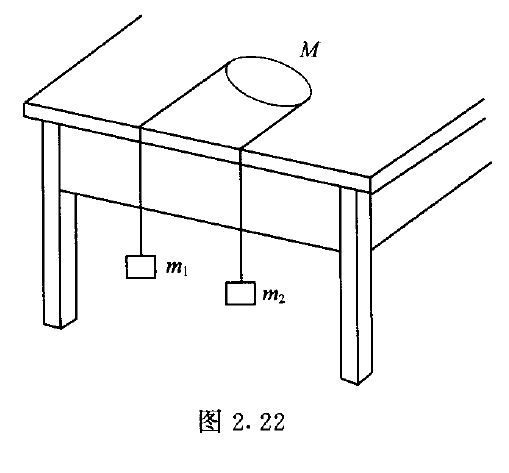
\includegraphics[width=0.4\textwidth]{image/2.22.JPG}
\end{figure}

\newpage


\begin{example} 
    $q_1$﹑$q_2$軸在豎直的xy平面內,與x軸的夾角分別為$\alpha$和$\beta$。一個拋射體在xy平面內運動,今取$q_1$﹑$q_2$為座標,給出或導出拋射體的運動微分方程。重力沿y軸的負方向。
    
    \rightline{[2.1.27]}
    
\end{example}

\begin{solution}
$\Ddot{q_1}cos\alpha + \Ddot{q_2}cos\beta = 0$\\
$\Ddot{q_1}sin\alpha + \Ddot{q_2}sin\beta = -g$\\
$\Ddot{q_1} = \frac{gcos\beta}{sin(\beta-\alpha)}$\\
$\Ddot{q_2} = \frac{gcos\alpha}{sin(\alpha-\beta}$
\end{solution}

\newpage


\begin{example} 
    質量分別為M和$M+m$的兩個人,分別拉住跨過定滑輪兩邊的繩子往上爬。開始時兩人與滑輪的距離都是h,都從靜止開始爬。設繩子不可伸長,繩子質量與繩子、滑輪間的摩擦力均可不計。證明:如質量較輕的人在t秒內爬到滑輪,這時質量較重的人與滑輪的距離為$\frac{m}{M+m}(h+\frac{1}{2}gt^2)$
    
    \rightline{[2.1.28]}
    
\end{example}

\begin{solution}

\end{solution}

\newpage


\begin{example} 
    一質量為m的跳水運動員,初速為零地從10m跳台上跳下。
    \begin{enumerate}[label=(\arabic*)]
    \item 求入水速度和從起跳到入水大致所用的時間;
    \item 假定作用在跳水者身上水的浮力和他所受的重力正好抵銷,作用在他身上的水的黏滯力大小為$bv^2$,試列出跳水員在水中垂直下沉的運動微分方程,以邊界條件$x=0$處$v=v_0$,求解速度v作為水面下深度x的函數;
    \item 若$\frac{b}{m} = 0.4m^{-1}$,求當$v = \frac{1}{10}v$時的深度;
    \item 求解跳水員在水下的垂直深度作為在水下的時間的函數。
    \end{enumerate}
    
    \rightline{[2.1.29]}
    
\end{example}

\begin{solution}
\begin{enumerate}[label=(\arabic*)]
\item $v = 14ms^(-1)$,$t = 1.43s$
\item $m\Ddot{x} = -b\Dot{x^2}$,$\Ddot{x} = \frac{d\Ddot{x}}{dx}\Dot{x}$\\
$m\Dot{x}\frac{d\Dot{x}}{dx} = -b\Dot{x^2}$,$\int_{v_0}^{v} \frac{1}{\Dot{x}}\, d\Dot{x} = -\int_{0}^{x} \frac{b}{m}\, dx$\\
$ln\frac{v}{v_0} = -\frac{b}{m}x$,$v = v_0e^{-\frac{b}{m}x}$
\item $x = 5.76m$
\item $x = \frac{m}{b}ln(1+\frac{bv_0}{m}t)$
\end{enumerate}
\end{solution}

\newpage


\begin{example} 
    一個質量為m的質點以初速v在y方向投射到沿x方向以不變速度V運動著的水平皮帶上並留在上面運動。若質點與皮帶間的滑動摩擦因數為$\mu$,質點接觸皮帶的初位置取為固定的xy坐標系的原點,求質點在皮帶上剛停止滑動時的xy座標。
    
    \rightline{[2.1.30]}
    
\end{example}

\begin{solution}

\end{solution}

\newpage


\begin{example} 
    在水平的xy平面內有一留聲機轉盤,他以恆定的角速度$\omega$繞過盤心的鉛垂軸旋轉。在轉盤上滑動的物體在水平方向受到兩個真實力作用:一個是大小為kr(r為質點至盤心的距離,k為常量),方向指向盤心的彈性力;另一個是摩擦力,與相對速度成正比,比例係數為c,c是正值常量,物體可視為質點。
    \begin{enumerate}[label=(\arabic*)]
    \item 如物體待在盤上任何位置均能相對轉盤保持靜止,問k有多大?
    \item 假設k是(1)問所得之值,在一般的初始條件下,求物體的相對速度$\Dot{x}$﹑$\Dot{y}$;
    \item 用(2)的結果進而求x(t)和y(t)。
    \end{enumerate}
    
    \rightline{[2.1.31]}
    
\end{example}

\begin{solution}
\begin{enumerate}[label=(\arabic*)]
\item $k = m\omega^2$
\item $\Dot{x} = e^{-\frac{c}{m}t}(\Dot{x_0}cos2\omega t + \Dot{y_0}sin2\omega t)$\\
$\Dot{y} = e^{-\frac{c}{m}t}(-\Dot{x_0}sin2\omega t + \Dot{y_0}cos2\omega t)$
\item $x = x_0 + \frac{m(c\Dot{x_0}+2m\omega \Dot{y_0})}{c^2+4m^2\omega^2} - \left[ \frac{m(c\Dot{x_0}+2m\omega \Dot{y_0})}{c^2+4m^2\omega^2}cos2\omega t - \frac{m(2m\omega \Dot{x_0} - c\Dot{y_0})}{c^2+4m^2\omega^2}sin2\omega t \right] e^{-\frac{c}{m}t}$ \\
$y = y_0 - \frac{m(2m\omega \Dot{x_0} - c \Dot{y_0})}{c^2+4m^2\omega^2} + \left[ \frac{m(2m\omega \Dot{x_0} - c \Dot{y_0})}{c^2+4m^2\omega^2}cos2\omega t - \frac{m(\Dot{x_0} + 2m\omega\Dot{y_0})}{c^2+4m^2\omega^2}sin2\omega t \right] e^{-\frac{c}{m}t}$
\end{enumerate}
\end{solution}

\newpage


\begin{example} 
    一個值點垂直上拋,初速為$v_0$,如空氣阻力與速率的平方成正比,證明:回到初始未至時的速率為$\frac{v_0v_t}{(v_0^2+v_t^2)^{1/2}}$,其中$v_t$是極限速率。
    
    \rightline{[2.1.32]}
    
\end{example}

\begin{solution}

\end{solution}

\newpage


\begin{example} 
    兩個質量均為m的質點A和B連在一個勁度係數為k的彈簧的兩端。開始兩質點靜放在光滑的水平面上,彈簧處於原長,然後沿AB方向給B以恆力ka。求兩質點的運動學方程。
    
    \rightline{[2.1.33]}
    
\end{example}

\begin{solution}
A:$x = \frac{1}{8}a\omega^2t^2 - \frac{1}{4}a(1-cos\omega t)$\\
B:$y = x + \frac{1}{2}a(1-cos\omega t) = \frac{1}{8}a\omega^2t^2 + \frac{1}{4}a(1-cos\omega t)$\\
其中$\omega^2 = \frac{2k}{m}$
\end{solution}

\newpage




















\end{document}